% Options for packages loaded elsewhere
\PassOptionsToPackage{unicode}{hyperref}
\PassOptionsToPackage{hyphens}{url}
%
\documentclass[
]{article}
\usepackage{lmodern}
\usepackage{amssymb,amsmath}
\usepackage{ifxetex,ifluatex}
\ifnum 0\ifxetex 1\fi\ifluatex 1\fi=0 % if pdftex
  \usepackage[T1]{fontenc}
  \usepackage[utf8]{inputenc}
  \usepackage{textcomp} % provide euro and other symbols
\else % if luatex or xetex
  \usepackage{unicode-math}
  \defaultfontfeatures{Scale=MatchLowercase}
  \defaultfontfeatures[\rmfamily]{Ligatures=TeX,Scale=1}
\fi
% Use upquote if available, for straight quotes in verbatim environments
\IfFileExists{upquote.sty}{\usepackage{upquote}}{}
\IfFileExists{microtype.sty}{% use microtype if available
  \usepackage[]{microtype}
  \UseMicrotypeSet[protrusion]{basicmath} % disable protrusion for tt fonts
}{}
\makeatletter
\@ifundefined{KOMAClassName}{% if non-KOMA class
  \IfFileExists{parskip.sty}{%
    \usepackage{parskip}
  }{% else
    \setlength{\parindent}{0pt}
    \setlength{\parskip}{6pt plus 2pt minus 1pt}}
}{% if KOMA class
  \KOMAoptions{parskip=half}}
\makeatother
\usepackage{xcolor}
\IfFileExists{xurl.sty}{\usepackage{xurl}}{} % add URL line breaks if available
\IfFileExists{bookmark.sty}{\usepackage{bookmark}}{\usepackage{hyperref}}
\hypersetup{
  pdftitle={Lab4},
  pdfauthor={Gege Qian, Andy Shi},
  hidelinks,
  pdfcreator={LaTeX via pandoc}}
\urlstyle{same} % disable monospaced font for URLs
\usepackage[margin=1in]{geometry}
\usepackage{color}
\usepackage{fancyvrb}
\newcommand{\VerbBar}{|}
\newcommand{\VERB}{\Verb[commandchars=\\\{\}]}
\DefineVerbatimEnvironment{Highlighting}{Verbatim}{commandchars=\\\{\}}
% Add ',fontsize=\small' for more characters per line
\usepackage{framed}
\definecolor{shadecolor}{RGB}{248,248,248}
\newenvironment{Shaded}{\begin{snugshade}}{\end{snugshade}}
\newcommand{\AlertTok}[1]{\textcolor[rgb]{0.94,0.16,0.16}{#1}}
\newcommand{\AnnotationTok}[1]{\textcolor[rgb]{0.56,0.35,0.01}{\textbf{\textit{#1}}}}
\newcommand{\AttributeTok}[1]{\textcolor[rgb]{0.77,0.63,0.00}{#1}}
\newcommand{\BaseNTok}[1]{\textcolor[rgb]{0.00,0.00,0.81}{#1}}
\newcommand{\BuiltInTok}[1]{#1}
\newcommand{\CharTok}[1]{\textcolor[rgb]{0.31,0.60,0.02}{#1}}
\newcommand{\CommentTok}[1]{\textcolor[rgb]{0.56,0.35,0.01}{\textit{#1}}}
\newcommand{\CommentVarTok}[1]{\textcolor[rgb]{0.56,0.35,0.01}{\textbf{\textit{#1}}}}
\newcommand{\ConstantTok}[1]{\textcolor[rgb]{0.00,0.00,0.00}{#1}}
\newcommand{\ControlFlowTok}[1]{\textcolor[rgb]{0.13,0.29,0.53}{\textbf{#1}}}
\newcommand{\DataTypeTok}[1]{\textcolor[rgb]{0.13,0.29,0.53}{#1}}
\newcommand{\DecValTok}[1]{\textcolor[rgb]{0.00,0.00,0.81}{#1}}
\newcommand{\DocumentationTok}[1]{\textcolor[rgb]{0.56,0.35,0.01}{\textbf{\textit{#1}}}}
\newcommand{\ErrorTok}[1]{\textcolor[rgb]{0.64,0.00,0.00}{\textbf{#1}}}
\newcommand{\ExtensionTok}[1]{#1}
\newcommand{\FloatTok}[1]{\textcolor[rgb]{0.00,0.00,0.81}{#1}}
\newcommand{\FunctionTok}[1]{\textcolor[rgb]{0.00,0.00,0.00}{#1}}
\newcommand{\ImportTok}[1]{#1}
\newcommand{\InformationTok}[1]{\textcolor[rgb]{0.56,0.35,0.01}{\textbf{\textit{#1}}}}
\newcommand{\KeywordTok}[1]{\textcolor[rgb]{0.13,0.29,0.53}{\textbf{#1}}}
\newcommand{\NormalTok}[1]{#1}
\newcommand{\OperatorTok}[1]{\textcolor[rgb]{0.81,0.36,0.00}{\textbf{#1}}}
\newcommand{\OtherTok}[1]{\textcolor[rgb]{0.56,0.35,0.01}{#1}}
\newcommand{\PreprocessorTok}[1]{\textcolor[rgb]{0.56,0.35,0.01}{\textit{#1}}}
\newcommand{\RegionMarkerTok}[1]{#1}
\newcommand{\SpecialCharTok}[1]{\textcolor[rgb]{0.00,0.00,0.00}{#1}}
\newcommand{\SpecialStringTok}[1]{\textcolor[rgb]{0.31,0.60,0.02}{#1}}
\newcommand{\StringTok}[1]{\textcolor[rgb]{0.31,0.60,0.02}{#1}}
\newcommand{\VariableTok}[1]{\textcolor[rgb]{0.00,0.00,0.00}{#1}}
\newcommand{\VerbatimStringTok}[1]{\textcolor[rgb]{0.31,0.60,0.02}{#1}}
\newcommand{\WarningTok}[1]{\textcolor[rgb]{0.56,0.35,0.01}{\textbf{\textit{#1}}}}
\usepackage{graphicx,grffile}
\makeatletter
\def\maxwidth{\ifdim\Gin@nat@width>\linewidth\linewidth\else\Gin@nat@width\fi}
\def\maxheight{\ifdim\Gin@nat@height>\textheight\textheight\else\Gin@nat@height\fi}
\makeatother
% Scale images if necessary, so that they will not overflow the page
% margins by default, and it is still possible to overwrite the defaults
% using explicit options in \includegraphics[width, height, ...]{}
\setkeys{Gin}{width=\maxwidth,height=\maxheight,keepaspectratio}
% Set default figure placement to htbp
\makeatletter
\def\fps@figure{htbp}
\makeatother
\setlength{\emergencystretch}{3em} % prevent overfull lines
\providecommand{\tightlist}{%
  \setlength{\itemsep}{0pt}\setlength{\parskip}{0pt}}
\setcounter{secnumdepth}{-\maxdimen} % remove section numbering

\title{Lab4}
\author{Gege Qian, Andy Shi}
\date{2/5/2021}

\begin{document}
\maketitle

\hypertarget{announcements}{%
\subsection{Announcements}\label{announcements}}

\begin{itemize}
\tightlist
\item
  HW2 is out, due 02/21/2021
\item
  By now, everyone should have a Cannon account
\end{itemize}

\hypertarget{outline}{%
\subsection{Outline}\label{outline}}

\begin{itemize}
\tightlist
\item
  PCA and Hierarchical Clustering
\item
  Batch Removal
\item
  DESeq2
\item
  KMeans
\item
  DAVID
\item
  GSEA
\item
  Next Week: Machine Learning and Modeling accuracy comparison \#\#
  Install and Load Packages
\end{itemize}

\begin{Shaded}
\begin{Highlighting}[]
\KeywordTok{library}\NormalTok{(sva)}
\KeywordTok{library}\NormalTok{(limma)}
\KeywordTok{library}\NormalTok{(bladderbatch)}
\KeywordTok{library}\NormalTok{(leukemiasEset)}
\KeywordTok{library}\NormalTok{(dplyr)}
\KeywordTok{library}\NormalTok{(biobroom)}
\KeywordTok{library}\NormalTok{(ggplot2)}
\KeywordTok{library}\NormalTok{(factoextra)}
\KeywordTok{library}\NormalTok{(purrr)}
\KeywordTok{setwd}\NormalTok{(}\StringTok{"."}\NormalTok{)}
\end{Highlighting}
\end{Shaded}

\hypertarget{pca}{%
\subsection{PCA}\label{pca}}

\begin{itemize}
\tightlist
\item
  Finds the best linear combinations of the variables.
\item
  ``Best'' means the variable that describes the largest variance
\item
  Can produce lower-dimensional summaries of the data.

  \begin{itemize}
  \tightlist
  \item
    Take 100 numbers per sample and summarize them with 2 numbers per
    sample.
  \end{itemize}
\item
  Useful for visualization, among other things.
  \includegraphics{PCA.gif}
\end{itemize}

\hypertarget{pca-analysis-example}{%
\subsection{PCA Analysis Example}\label{pca-analysis-example}}

We'll use the data sets decathlon2 {[}in factoextra{]}

Briefly, it contains:

Active individuals (rows 1 to 23) and active variables (columns 1 to
10), which are used to perform the principal component analysis
Supplementary individuals (rows 24 to 27) and supplementary variables
(columns 11 to 13), which coordinates will be predicted using the PCA
information and parameters obtained with active individuals/variables.

\begin{Shaded}
\begin{Highlighting}[]
\KeywordTok{data}\NormalTok{(decathlon2)}
\NormalTok{decathlon2.active <-}\StringTok{ }\NormalTok{decathlon2[}\DecValTok{1}\OperatorTok{:}\DecValTok{23}\NormalTok{, }\DecValTok{1}\OperatorTok{:}\DecValTok{10}\NormalTok{]}
\KeywordTok{head}\NormalTok{(decathlon2.active[, }\DecValTok{1}\OperatorTok{:}\DecValTok{6}\NormalTok{])}
\end{Highlighting}
\end{Shaded}

\begin{verbatim}
##           X100m Long.jump Shot.put High.jump X400m X110m.hurdle
## SEBRLE    11.04      7.58    14.83      2.07 49.81        14.69
## CLAY      10.76      7.40    14.26      1.86 49.37        14.05
## BERNARD   11.02      7.23    14.25      1.92 48.93        14.99
## YURKOV    11.34      7.09    15.19      2.10 50.42        15.31
## ZSIVOCZKY 11.13      7.30    13.48      2.01 48.62        14.17
## McMULLEN  10.83      7.31    13.76      2.13 49.91        14.38
\end{verbatim}

\begin{Shaded}
\begin{Highlighting}[]
\NormalTok{res.pca <-}\StringTok{ }\KeywordTok{prcomp}\NormalTok{(decathlon2.active, }\DataTypeTok{scale =} \OtherTok{TRUE}\NormalTok{)}
\NormalTok{pca.var.per =}\StringTok{ }\KeywordTok{round}\NormalTok{(res.pca}\OperatorTok{$}\NormalTok{sdev}\OperatorTok{^}\DecValTok{2}\OperatorTok{/}\KeywordTok{sum}\NormalTok{(res.pca}\OperatorTok{$}\NormalTok{sdev}\OperatorTok{^}\DecValTok{2}\NormalTok{)}\OperatorTok{*}\DecValTok{100}\NormalTok{,}\DecValTok{1}\NormalTok{)}
\KeywordTok{fviz_eig}\NormalTok{(res.pca, }\DataTypeTok{addlabels=}\OtherTok{TRUE}\NormalTok{, }\DataTypeTok{ylim=}\KeywordTok{c}\NormalTok{(}\DecValTok{0}\NormalTok{,}\DecValTok{100}\NormalTok{), }\DataTypeTok{geom =} \KeywordTok{c}\NormalTok{(}\StringTok{"bar"}\NormalTok{, }\StringTok{"line"}\NormalTok{), }\DataTypeTok{barfill =} \StringTok{"gold"}\NormalTok{, }\DataTypeTok{barcolor=}\StringTok{"grey"}\NormalTok{,}\DataTypeTok{linecolor =} \StringTok{"red"}\NormalTok{, }\DataTypeTok{ncp=}\DecValTok{10}\NormalTok{)}\OperatorTok{+}
\KeywordTok{labs}\NormalTok{(}\DataTypeTok{title =} \StringTok{"PCA Coverage"}\NormalTok{,}
         \DataTypeTok{x =} \StringTok{"Principal Components"}\NormalTok{, }\DataTypeTok{y =} \StringTok{"% of variances"}\NormalTok{)}
\end{Highlighting}
\end{Shaded}

\includegraphics{Lab4_files/figure-latex/pca-1.pdf}

\begin{Shaded}
\begin{Highlighting}[]
\NormalTok{ggplot_data <-}\StringTok{ }\KeywordTok{data.frame}\NormalTok{(}\DataTypeTok{Sample =} \KeywordTok{rownames}\NormalTok{(res.pca}\OperatorTok{$}\NormalTok{x),}\DataTypeTok{X =}\NormalTok{ res.pca}\OperatorTok{$}\NormalTok{x[,}\DecValTok{1}\NormalTok{], }\DataTypeTok{Y =}\NormalTok{ res.pca}\OperatorTok{$}\NormalTok{x[,}\DecValTok{2}\NormalTok{]) }
\NormalTok{run<-}\KeywordTok{c}\NormalTok{()}
\NormalTok{run[decathlon2.active}\OperatorTok{$}\NormalTok{X100m}\OperatorTok{<}\DecValTok{11}\NormalTok{]<-}\StringTok{"slow"}
\NormalTok{run[decathlon2.active}\OperatorTok{$}\NormalTok{X100m}\OperatorTok{>=}\DecValTok{11}\NormalTok{]<-}\StringTok{"fast"}
\KeywordTok{names}\NormalTok{(run)<-}\KeywordTok{rownames}\NormalTok{(decathlon2.active)}
\KeywordTok{ggplot}\NormalTok{(}\DataTypeTok{data =}\NormalTok{ ggplot_data,}\KeywordTok{aes}\NormalTok{(}\DataTypeTok{x=}\NormalTok{X,}\DataTypeTok{y=}\NormalTok{Y,}\DataTypeTok{label =}\NormalTok{Sample, }\DataTypeTok{color=}\NormalTok{run))}\OperatorTok{+}
\StringTok{  }\KeywordTok{geom_point}\NormalTok{()}\OperatorTok{+}
\StringTok{  }\KeywordTok{xlab}\NormalTok{(}\KeywordTok{paste}\NormalTok{(}\StringTok{"PC1-"}\NormalTok{,pca.var.per[}\DecValTok{1}\NormalTok{],}\StringTok{"%"}\NormalTok{,}\DataTypeTok{sep =}\StringTok{" "}\NormalTok{))}\OperatorTok{+}
\StringTok{  }\KeywordTok{ylab}\NormalTok{(}\KeywordTok{paste}\NormalTok{(}\StringTok{"PC2-"}\NormalTok{,pca.var.per[}\DecValTok{2}\NormalTok{],}\StringTok{"%"}\NormalTok{,}\DataTypeTok{sep =}\StringTok{" "}\NormalTok{))}\OperatorTok{+}
\StringTok{  }\KeywordTok{theme_bw}\NormalTok{()}\OperatorTok{+}
\StringTok{  }\KeywordTok{ggtitle}\NormalTok{(}\StringTok{"PCA graph of the first two components"}\NormalTok{)}
\end{Highlighting}
\end{Shaded}

\includegraphics{Lab4_files/figure-latex/pca-2.pdf}

\hypertarget{r-aside-lists}{%
\subsection{R Aside: Lists}\label{r-aside-lists}}

\begin{itemize}
\tightlist
\item
  \texttt{pca\_result} is a list. It holds a mix of data types.
\item
  Can access an individual list element with \texttt{\$},
  e.g.~\texttt{pca\_result\$x}.
\item
  A lot of R functions use lists to return multiple things.
\item
  Look at \texttt{prcomp} documentation (\texttt{?prcomp}) under Value
  to see the meaning of each of the things in the list.
\end{itemize}

\hypertarget{pca-variance-explained}{%
\subsection{PCA Variance Explained}\label{pca-variance-explained}}

\begin{itemize}
\tightlist
\item
  Linear algebra result: \(\text{trace}(\Sigma) = \sum_i \lambda_i\)
\item
  \(\text{trace}(\Sigma)\) can be thought of as total variance.
\item
  Variance of \(PC_i\) is \(\lambda_i\)
\item
  So variance explained by PCs 1 to j is
  \(\frac{\sum_{i = 1}^j \lambda_i}{\sum_{i = 1}^K \lambda_i}\)
\item
  Denominator is sum of all eigenvalues
\end{itemize}

\hypertarget{kmeans}{%
\subsection{KMeans}\label{kmeans}}

\begin{itemize}
\tightlist
\item
  An unsupervised method to cluster the data (no labels/outcomes
  provided).
\item
  Requires that you specify the number of clusters in advance.
\item
  We can use either all the genes, or only the differently expressed
  genes.
\end{itemize}

\hypertarget{data-preparation}{%
\subsubsection{Data Preparation}\label{data-preparation}}

\begin{itemize}
\tightlist
\item
  Rows are observations (individuals) and columns are variables
\item
  Any missing value in the data must be removed or estimated.
\item
  The data must be standardized (i.e., scaled) to make variables
  comparable. Recall that, standardization consists of transforming the
  variables such that they have mean zero and standard deviation one
  \includegraphics{k-means.gif}
\end{itemize}

\begin{Shaded}
\begin{Highlighting}[]
\NormalTok{df <-}\StringTok{ }\NormalTok{USArrests}
\NormalTok{df <-}\StringTok{ }\KeywordTok{na.omit}\NormalTok{(df)}
\NormalTok{df <-}\StringTok{ }\KeywordTok{scale}\NormalTok{(df)}
\NormalTok{distance <-}\StringTok{ }\KeywordTok{get_dist}\NormalTok{(df)}
\KeywordTok{fviz_dist}\NormalTok{(distance, }\DataTypeTok{gradient =} \KeywordTok{list}\NormalTok{(}\DataTypeTok{low =} \StringTok{"#00AFBB"}\NormalTok{, }\DataTypeTok{mid =} \StringTok{"white"}\NormalTok{, }\DataTypeTok{high =} \StringTok{"#FC4E07"}\NormalTok{))}
\end{Highlighting}
\end{Shaded}

\includegraphics{Lab4_files/figure-latex/k-means-1.pdf}

\begin{Shaded}
\begin{Highlighting}[]
\NormalTok{k2 <-}\StringTok{ }\KeywordTok{kmeans}\NormalTok{(df, }\DataTypeTok{centers =} \DecValTok{2}\NormalTok{, }\DataTypeTok{nstart =} \DecValTok{25}\NormalTok{)}
\KeywordTok{fviz_cluster}\NormalTok{(k2, }\DataTypeTok{data =}\NormalTok{ df)}
\end{Highlighting}
\end{Shaded}

\includegraphics{Lab4_files/figure-latex/k-means-2.pdf}

\begin{Shaded}
\begin{Highlighting}[]
\NormalTok{k3 <-}\StringTok{ }\KeywordTok{kmeans}\NormalTok{(df, }\DataTypeTok{centers =} \DecValTok{3}\NormalTok{, }\DataTypeTok{nstart =} \DecValTok{25}\NormalTok{)}
\NormalTok{k4 <-}\StringTok{ }\KeywordTok{kmeans}\NormalTok{(df, }\DataTypeTok{centers =} \DecValTok{4}\NormalTok{, }\DataTypeTok{nstart =} \DecValTok{25}\NormalTok{)}
\NormalTok{k5 <-}\StringTok{ }\KeywordTok{kmeans}\NormalTok{(df, }\DataTypeTok{centers =} \DecValTok{5}\NormalTok{, }\DataTypeTok{nstart =} \DecValTok{25}\NormalTok{)}

\CommentTok{# plots to compare}
\NormalTok{p1 <-}\StringTok{ }\KeywordTok{fviz_cluster}\NormalTok{(k2, }\DataTypeTok{geom =} \StringTok{"point"}\NormalTok{, }\DataTypeTok{data =}\NormalTok{ df) }\OperatorTok{+}\StringTok{ }\KeywordTok{ggtitle}\NormalTok{(}\StringTok{"k = 2"}\NormalTok{)}
\NormalTok{p2 <-}\StringTok{ }\KeywordTok{fviz_cluster}\NormalTok{(k3, }\DataTypeTok{geom =} \StringTok{"point"}\NormalTok{,  }\DataTypeTok{data =}\NormalTok{ df) }\OperatorTok{+}\StringTok{ }\KeywordTok{ggtitle}\NormalTok{(}\StringTok{"k = 3"}\NormalTok{)}
\NormalTok{p3 <-}\StringTok{ }\KeywordTok{fviz_cluster}\NormalTok{(k4, }\DataTypeTok{geom =} \StringTok{"point"}\NormalTok{,  }\DataTypeTok{data =}\NormalTok{ df) }\OperatorTok{+}\StringTok{ }\KeywordTok{ggtitle}\NormalTok{(}\StringTok{"k = 4"}\NormalTok{)}
\NormalTok{p4 <-}\StringTok{ }\KeywordTok{fviz_cluster}\NormalTok{(k5, }\DataTypeTok{geom =} \StringTok{"point"}\NormalTok{,  }\DataTypeTok{data =}\NormalTok{ df) }\OperatorTok{+}\StringTok{ }\KeywordTok{ggtitle}\NormalTok{(}\StringTok{"k = 5"}\NormalTok{)}

\KeywordTok{library}\NormalTok{(gridExtra)}
\end{Highlighting}
\end{Shaded}

\begin{verbatim}
## 
## Attaching package: 'gridExtra'
\end{verbatim}

\begin{verbatim}
## The following object is masked from 'package:dplyr':
## 
##     combine
\end{verbatim}

\begin{verbatim}
## The following object is masked from 'package:Biobase':
## 
##     combine
\end{verbatim}

\begin{verbatim}
## The following object is masked from 'package:BiocGenerics':
## 
##     combine
\end{verbatim}

\begin{Shaded}
\begin{Highlighting}[]
\KeywordTok{grid.arrange}\NormalTok{(p1, p2, p3, p4, }\DataTypeTok{nrow =} \DecValTok{2}\NormalTok{)}
\end{Highlighting}
\end{Shaded}

\includegraphics{Lab4_files/figure-latex/k-means2-1.pdf}

\begin{Shaded}
\begin{Highlighting}[]
\KeywordTok{set.seed}\NormalTok{(}\DecValTok{123}\NormalTok{)}

\CommentTok{# function to compute total within-cluster sum of square }
\NormalTok{wss <-}\StringTok{ }\ControlFlowTok{function}\NormalTok{(k) \{}
  \KeywordTok{kmeans}\NormalTok{(df, k, }\DataTypeTok{nstart =} \DecValTok{10}\NormalTok{ )}\OperatorTok{$}\NormalTok{tot.withinss}
\NormalTok{\}}

\CommentTok{# Compute and plot wss for k = 1 to k = 15}
\NormalTok{k.values <-}\StringTok{ }\DecValTok{1}\OperatorTok{:}\DecValTok{15}

\CommentTok{# extract wss for 2-15 clusters}
\NormalTok{wss_values <-}\StringTok{ }\KeywordTok{map_dbl}\NormalTok{(k.values, wss)}

\KeywordTok{plot}\NormalTok{(k.values, wss_values,}
       \DataTypeTok{type=}\StringTok{"b"}\NormalTok{, }\DataTypeTok{pch =} \DecValTok{19}\NormalTok{, }\DataTypeTok{frame =} \OtherTok{FALSE}\NormalTok{, }
       \DataTypeTok{xlab=}\StringTok{"Number of clusters K"}\NormalTok{,}
       \DataTypeTok{ylab=}\StringTok{"Total within-clusters sum of squares"}\NormalTok{)}
\end{Highlighting}
\end{Shaded}

\includegraphics{Lab4_files/figure-latex/k-means2-2.pdf} \#\#
Hierarchical Clustering - Hierarchical clustering is an alternative
approach to k-means clustering for identifying groups in the dataset -
Dose not pre-specify the number of clusters - Generate tree-based
representation of the observations, called a dendrogram.

\begin{Shaded}
\begin{Highlighting}[]
\NormalTok{d <-}\StringTok{ }\KeywordTok{dist}\NormalTok{(df, }\DataTypeTok{method =} \StringTok{"euclidean"}\NormalTok{)}

\CommentTok{# Hierarchical clustering using Complete Linkage}
\NormalTok{hc1 <-}\StringTok{ }\KeywordTok{hclust}\NormalTok{(d, }\DataTypeTok{method =} \StringTok{"complete"}\NormalTok{ )}

\CommentTok{# Plot the obtained dendrogram}
\KeywordTok{plot}\NormalTok{(hc1, }\DataTypeTok{cex =} \FloatTok{0.6}\NormalTok{, }\DataTypeTok{hang =} \DecValTok{-1}\NormalTok{)}
\end{Highlighting}
\end{Shaded}

\includegraphics{Lab4_files/figure-latex/heriarchecal clustering-1.pdf}

\hypertarget{batch-effect}{%
\subsection{Batch Effect}\label{batch-effect}}

\begin{itemize}
\tightlist
\item
  Why is batch effect a problem?
\item
  Example data: Gene expression data from investigation into bladder
  cancer.
\item
  Outcome: finding differentially expressed genes that are associated
  with cancer status (0/1 in the variable \texttt{hasCancer}).
\item
  Already normalized with RMA.
\item
  \texttt{pheno}: Dataset that contains phenotypes.
\item
  \texttt{edata}: Expression matrix.
\end{itemize}

\begin{Shaded}
\begin{Highlighting}[]
\KeywordTok{data}\NormalTok{(bladderdata)}
\NormalTok{pheno <-}\StringTok{ }\KeywordTok{pData}\NormalTok{(bladderEset)}
\NormalTok{pheno <-}\StringTok{ }\NormalTok{pheno }\OperatorTok
\StringTok{    }\KeywordTok{mutate}\NormalTok{(}\DataTypeTok{hasCancer =} \KeywordTok{as.numeric}\NormalTok{(cancer }\OperatorTok{==}\StringTok{ "Cancer"}\NormalTok{))}
\KeywordTok{head}\NormalTok{(pheno)}
\end{Highlighting}
\end{Shaded}

\begin{verbatim}
##   sample outcome batch cancer hasCancer
## 1      1  Normal     3 Normal         0
## 2      2  Normal     2 Normal         0
## 3      3  Normal     2 Normal         0
## 4      4  Normal     3 Normal         0
## 5      5  Normal     3 Normal         0
## 6      6  Normal     3 Normal         0
\end{verbatim}

\begin{Shaded}
\begin{Highlighting}[]
\NormalTok{edata <-}\StringTok{ }\KeywordTok{exprs}\NormalTok{(bladderEset)}
\end{Highlighting}
\end{Shaded}

\begin{Shaded}
\begin{Highlighting}[]
\NormalTok{expr.dat <-}\StringTok{ }\KeywordTok{t}\NormalTok{(edata)}
\CommentTok{#expr.dat <- t(log2(tpm+1))}

\CommentTok{### PCA: before batch effect}
\NormalTok{PCA1 <-}\StringTok{ }\KeywordTok{prcomp}\NormalTok{(expr.dat)}\OperatorTok{$}\NormalTok{x}
\NormalTok{df1 <-}\StringTok{ }\KeywordTok{cbind.data.frame}\NormalTok{(PCA1,}\DataTypeTok{batch =} \KeywordTok{factor}\NormalTok{(pheno}\OperatorTok{$}\NormalTok{batch),}
                        \DataTypeTok{cancer =} \KeywordTok{factor}\NormalTok{(pheno}\OperatorTok{$}\NormalTok{cancer))}
\CommentTok{###plot}
\KeywordTok{ggplot}\NormalTok{(df1, }\KeywordTok{aes}\NormalTok{(}\DataTypeTok{x =}\NormalTok{ PC1, }\DataTypeTok{y =}\NormalTok{ PC2, }\DataTypeTok{shape =}\NormalTok{ cancer, }\DataTypeTok{color =}\NormalTok{ batch)) }\OperatorTok{+}\StringTok{ }
\StringTok{  }\KeywordTok{geom_point}\NormalTok{(}\DataTypeTok{size=}\DecValTok{3}\NormalTok{) }\OperatorTok{+}\StringTok{ }
\StringTok{  }\KeywordTok{labs}\NormalTok{(}\DataTypeTok{title=}\StringTok{"Before Batch effect removal"}\NormalTok{)}\OperatorTok{+}\StringTok{ }
\StringTok{  }\KeywordTok{theme_bw}\NormalTok{()}
\end{Highlighting}
\end{Shaded}

\includegraphics{Lab4_files/figure-latex/clustering-1.pdf}

\begin{Shaded}
\begin{Highlighting}[]
\NormalTok{temp <-}\StringTok{ }\NormalTok{expr.dat}
\KeywordTok{rownames}\NormalTok{(temp) <-}\StringTok{ }\KeywordTok{paste}\NormalTok{(}\KeywordTok{rownames}\NormalTok{(expr.dat), }\KeywordTok{as.character}\NormalTok{(pheno}\OperatorTok{$}\NormalTok{batch), }\DataTypeTok{sep =} \StringTok{"_"}\NormalTok{)}
\NormalTok{dd <-}\StringTok{ }\KeywordTok{dist}\NormalTok{(}\KeywordTok{scale}\NormalTok{(temp), }\DataTypeTok{method =} \StringTok{"euclidean"}\NormalTok{)}
\NormalTok{hc <-}\StringTok{ }\KeywordTok{hclust}\NormalTok{(dd, }\DataTypeTok{method =} \StringTok{"ward.D2"}\NormalTok{)}
\KeywordTok{plot}\NormalTok{(hc, }\DataTypeTok{hang =} \DecValTok{-1}\NormalTok{, }\DataTypeTok{cex =} \FloatTok{0.6}\NormalTok{, }\DataTypeTok{main =} \StringTok{"Before batch effect removal"}\NormalTok{)}
\end{Highlighting}
\end{Shaded}

\includegraphics{Lab4_files/figure-latex/clustering-2.pdf}

\hypertarget{combat}{%
\subsection{ComBat}\label{combat}}

\begin{itemize}
\tightlist
\item
  Perform batch effect adjustment
\item
  Need to specify model matrix: same matrix you use for LIMMA
\item
  Tells ComBat to remove the batch effect but not to remove the
  association due to whatever model you are going to run.
\item
  In this example, we model gene expression as a function of whether or
  not the sample is cancerous (\texttt{hasCancer} variable)
\end{itemize}

\begin{Shaded}
\begin{Highlighting}[]
\NormalTok{model <-}\StringTok{ }\KeywordTok{model.matrix}\NormalTok{(}\OperatorTok{~}\NormalTok{pheno}\OperatorTok{$}\NormalTok{hasCancer)}
\NormalTok{combat_edata <-}\StringTok{ }\KeywordTok{ComBat}\NormalTok{(}\DataTypeTok{dat =}\NormalTok{ edata, }\DataTypeTok{batch =}\NormalTok{ pheno}\OperatorTok{$}\NormalTok{batch, }\DataTypeTok{mod =}\NormalTok{ model)}
\end{Highlighting}
\end{Shaded}

\begin{verbatim}
## Found5batches
\end{verbatim}

\begin{verbatim}
## Adjusting for1covariate(s) or covariate level(s)
\end{verbatim}

\begin{verbatim}
## Standardizing Data across genes
\end{verbatim}

\begin{verbatim}
## Fitting L/S model and finding priors
\end{verbatim}

\begin{verbatim}
## Finding parametric adjustments
\end{verbatim}

\begin{verbatim}
## Adjusting the Data
\end{verbatim}

\hypertarget{check-clustering-again}{%
\subsection{Check Clustering Again}\label{check-clustering-again}}

\begin{itemize}
\tightlist
\item
  Can you perform clustering to check whether ComBat removed the batch
  effect?
\end{itemize}

\begin{Shaded}
\begin{Highlighting}[]
\NormalTok{expr.combat <-}\StringTok{ }\KeywordTok{t}\NormalTok{(combat_edata)}

\CommentTok{###PCA: after batch effect removal}
\NormalTok{PCA2 <-}\StringTok{ }\KeywordTok{prcomp}\NormalTok{(expr.combat)}\OperatorTok{$}\NormalTok{x}
\NormalTok{df2 <-}\StringTok{ }\KeywordTok{cbind.data.frame}\NormalTok{(PCA2,}
                        \DataTypeTok{batch =} \KeywordTok{factor}\NormalTok{(pheno}\OperatorTok{$}\NormalTok{batch),}
                        \DataTypeTok{tissue =} \KeywordTok{factor}\NormalTok{(pheno}\OperatorTok{$}\NormalTok{cancer))}
\CommentTok{###plot}
\KeywordTok{ggplot}\NormalTok{(df2, }\KeywordTok{aes}\NormalTok{(}\DataTypeTok{x =}\NormalTok{ PC1, }\DataTypeTok{y =}\NormalTok{ PC2, }\DataTypeTok{shape =}\NormalTok{ tissue, }\DataTypeTok{color =}\NormalTok{ batch)) }\OperatorTok{+}
\StringTok{  }\KeywordTok{geom_point}\NormalTok{(}\DataTypeTok{size=}\DecValTok{3}\NormalTok{) }\OperatorTok{+}
\StringTok{  }\KeywordTok{labs}\NormalTok{(}\DataTypeTok{title=}\StringTok{"After Batch effect removal"}\NormalTok{)}\OperatorTok{+}
\StringTok{  }\KeywordTok{theme_bw}\NormalTok{()}
\end{Highlighting}
\end{Shaded}

\includegraphics{Lab4_files/figure-latex/combat-clusters-1.pdf}

\hypertarget{david-vs.-gsea}{%
\subsection{DAVID vs.~GSEA}\label{david-vs.-gsea}}

\begin{itemize}
\tightlist
\item
  Idea: look for sets of genes (e.g.~biological pathways) that are
  overrepresented in your results.
\item
  DAVID takes a selected list of differentially expressed genes and sees
  if there are genes in certain gene sets that are over-represented by
  counting.
\item
  GSEA takes all the genes and uses the test statistics (e.g.~t-value).
\item
  Need to have a good definition for the gene set.
\item
  DAVID has its own gene set definitions.
\item
  GSEA requires you to supply your own---can choose many different ones.

  \begin{itemize}
  \tightlist
  \item
    One good option is
    \href{http://software.broadinstitute.org/gsea/msigdb/index.jsp}{MSigDB}.
  \item
    Curated gene sets from the Broad Institute for many organisms.
  \item
    We will use the Hallmark gene set for humans.
  \end{itemize}
\end{itemize}

\hypertarget{david}{%
\subsection{DAVID}\label{david}}

\begin{itemize}
\tightlist
\item
  Take differentially expressed genes from limma.
\item
  Upload tab:

  \begin{enumerate}
  \def\labelenumi{\arabic{enumi}.}
  \tightlist
  \item
    Paste list into DAVID.
  \item
    Select identifier: AFFYMETRIX\_3PRIME\_IVT\_ID
  \item
    List type: check gene list.
  \item
    Submit
  \end{enumerate}
\item
  Background tab: select the Affymetrix array that was used.

  \begin{itemize}
  \tightlist
  \item
    For the bladder data and for HW, it's Human Genome U133 Plus 2
    Array.
  \end{itemize}
\item
  Functional annotation clustering.
\end{itemize}

\begin{Shaded}
\begin{Highlighting}[]
\NormalTok{design <-}\StringTok{ }\KeywordTok{model.matrix}\NormalTok{(}\OperatorTok{~}\NormalTok{pheno}\OperatorTok{$}\NormalTok{hasCancer)}
\NormalTok{limma_fit <-}\StringTok{ }\KeywordTok{lmFit}\NormalTok{(combat_edata, design) }\OperatorTok
\StringTok{    }\KeywordTok{eBayes}\NormalTok{() }\OperatorTok
\StringTok{    }\KeywordTok{tidy}\NormalTok{() }\OperatorTok
\StringTok{    }\KeywordTok{mutate}\NormalTok{(}\DataTypeTok{fdr =} \KeywordTok{p.adjust}\NormalTok{(p.value, }\DataTypeTok{method =} \StringTok{"fdr"}\NormalTok{)) }\OperatorTok
\StringTok{    }\KeywordTok{arrange}\NormalTok{(p.value)}
\end{Highlighting}
\end{Shaded}

\begin{verbatim}
## Warning: `tbl_df()` is deprecated as of dplyr 1.0.0.
## Please use `tibble::as_tibble()` instead.
## This warning is displayed once every 8 hours.
## Call `lifecycle::last_warnings()` to see where this warning was generated.
\end{verbatim}

\begin{Shaded}
\begin{Highlighting}[]
\NormalTok{up_genes <-}\StringTok{ }\NormalTok{limma_fit }\OperatorTok\StringTok{ }\KeywordTok{filter}\NormalTok{(fdr }\OperatorTok{<}\StringTok{ }\FloatTok{0.05}\NormalTok{, estimate }\OperatorTok{>}\StringTok{ }\KeywordTok{log2}\NormalTok{(}\DecValTok{2}\NormalTok{))}
\NormalTok{down_genes <-}\StringTok{ }\NormalTok{limma_fit }\OperatorTok\StringTok{ }\KeywordTok{filter}\NormalTok{(fdr }\OperatorTok{<}\StringTok{ }\FloatTok{0.05}\NormalTok{, estimate }\OperatorTok{<}\StringTok{ }\OperatorTok{-}\KeywordTok{log2}\NormalTok{(}\DecValTok{2}\NormalTok{))}
\KeywordTok{write.csv}\NormalTok{(up_genes, }\DataTypeTok{file =} \StringTok{"david_up.csv"}\NormalTok{)}
\KeywordTok{write.csv}\NormalTok{(down_genes, }\DataTypeTok{file =} \StringTok{"david_down.csv"}\NormalTok{)}
\end{Highlighting}
\end{Shaded}

\hypertarget{gsea}{%
\subsection{GSEA}\label{gsea}}

The list of differentially expressed genes is sometimes so long that its
interpretation becomes cumbersome and time consuming. A common
downstream procedure is gene set testing. It aims to understand which
pathways or gene networks the deferentially expressed genes are
implicated in.

\hypertarget{gsea-analysis}{%
\subsubsection{GSEA analysis}\label{gsea-analysis}}

\begin{itemize}
\tightlist
\item
  ranking all genes in the data set
\item
  identifying the rank positions of all members of the gene set in the
  ranked data set
\item
  calculating an enrichment score (ES) that represents the difference
  between the observed rankings and that which would be expected
  assuming a random rank distribution. \#\#\#\# Create Rank List
\end{itemize}

\begin{Shaded}
\begin{Highlighting}[]
\NormalTok{gseaDat <-}\StringTok{ }\KeywordTok{filter}\NormalTok{(shrinkLvV, }\OperatorTok{!}\KeywordTok{is.na}\NormalTok{(Entrez))}
\NormalTok{ranks <-}\StringTok{ }\NormalTok{gseaDat}\OperatorTok{$}\NormalTok{logFC}
\KeywordTok{names}\NormalTok{(ranks) <-}\StringTok{ }\NormalTok{gseaDat}\OperatorTok{$}\NormalTok{Entrez}
\KeywordTok{head}\NormalTok{(ranks)}
\KeywordTok{barplot}\NormalTok{(}\KeywordTok{sort}\NormalTok{(ranks, }\DataTypeTok{decreasing =}\NormalTok{ T))}
\end{Highlighting}
\end{Shaded}

\begin{figure}
\centering
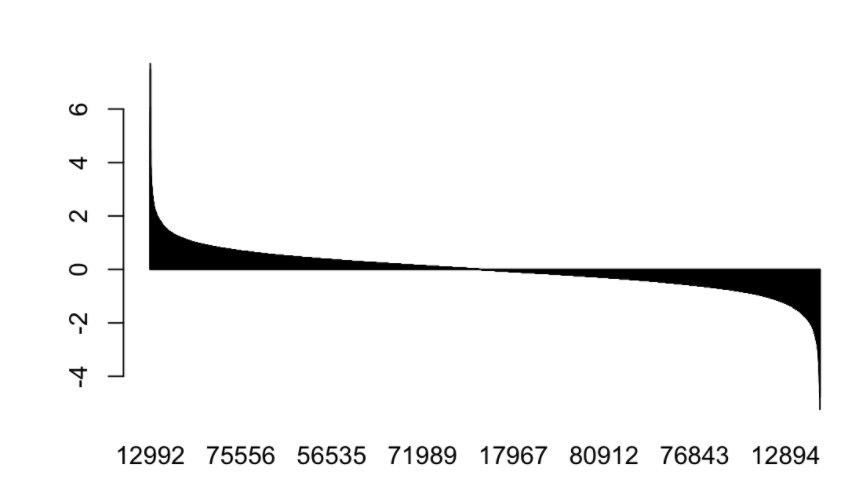
\includegraphics{rank.png}
\caption{Rank}
\end{figure}

\begin{Shaded}
\begin{Highlighting}[]
\NormalTok{fgseaRes <-}\StringTok{ }\KeywordTok{fgsea}\NormalTok{(pathwaysH, ranks, }\DataTypeTok{minSize=}\DecValTok{15}\NormalTok{, }\DataTypeTok{maxSize =} \DecValTok{500}\NormalTok{, }\DataTypeTok{nperm=}\DecValTok{1000}\NormalTok{)}
\KeywordTok{head}\NormalTok{(fgseaRes[}\KeywordTok{order}\NormalTok{(padj, }\OperatorTok{-}\KeywordTok{abs}\NormalTok{(NES)), ], }\DataTypeTok{n=}\DecValTok{10}\NormalTok{)}
\KeywordTok{plotEnrichment}\NormalTok{(pathwaysH[[}\StringTok{"HALLMARK_ESTROGEN_RESPONSE_EARLY"}\NormalTok{]], ranks)}
\end{Highlighting}
\end{Shaded}

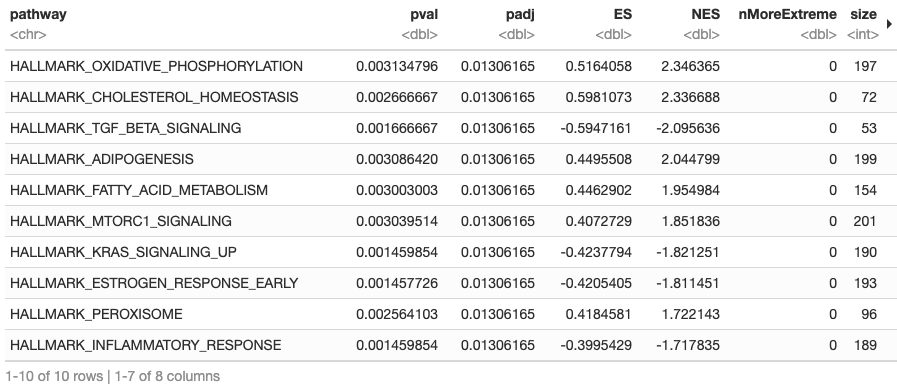
\includegraphics{GSEA2.png} 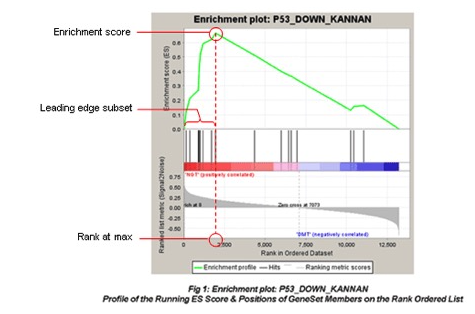
\includegraphics{gsea4.png} ● The top
portion of the plot shows the running ES for the gene set as the
analysis walks down the ranked list. The score at the peak of the plot
(the score furthest from 0.0) is the ES for the gene set. Gene sets with
a distinct peak at the beginning (such as the one shown here) or end of
the ranked list are generally the most interesting.

● The middle portion of the plot shows where the members of the gene set
appear in the ranked list of genes.

The leading edge subset of a gene set is the subset of members that
contribute most to the ES. For a positive ES (such as the one shown
here), the leading edge subset is the set of members that appear in the
ranked list prior to the peak score. For a negative ES, it is the set of
members that appear subsequent to the peak score.

● The bottom portion of the plot shows the value of the ranking metric
as you move down the list of ranked genes. The ranking metric measures a
gene's correlation with a phenotype. The value of the ranking metric
goes from positive to negative as you move down the ranked list. A
positive value indicates correlation with the first phenotype and a
negative value indicates correlation with the second phenotype. For
continuous phenotypes (time series or gene of interest), a positive
value indicates correlation with the phenotype profile and a negative
value indicates no correlation or inverse correlation with the profile.

\end{document}
